\documentclass[a4paper,twoside]{article}

\usepackage{epsfig}
\usepackage{graphicx}
\usepackage{subcaption}
\usepackage{calc}
\usepackage{amssymb}
\usepackage{amstext}
\usepackage{amsmath}
\usepackage{amsthm}
\usepackage{multicol}
\usepackage{pslatex}
\usepackage{natbib}
\usepackage{algorithm2e}
\usepackage[bottom]{footmisc}
\usepackage{SCITEPRESS}     % Please add other packages that you may need BEFORE the SCITEPRESS.sty package.
\usepackage[hidelinks]{hyperref}

\begin{document}

\title{Transforming Mentorship: A Hybrid Retrieval-Augmented Generation Architecture for Academic Advising}

\author{\authorname{Anonymous Author(s)}
\affiliation{Anonymous Institute}
\email{anonymous@anonymous.edu}
}

\keywords{Chatbot, Retrieval-Augmented Generation, Hybrid Retrieval, Academic Advising, Hallucination Detection, Natural Language Processing, Educational Technology, Information Retrieval.}

\abstract{University students in open-credit systems face persistent barriers to timely academic guidance, including limited mentor availability, complex and frequently updated policy information, and scheduling constraints. We present a retrieval-augmented chatbot that combines BM25 lexical retrieval with ChromaDB semantic retrieval to answer academic advising queries, using a locally hosted Llama-3.1-8B model for response generation over an academic-advising corpus drawn from institutional spreadsheets and student community forums. We evaluate the system along three axes: semantic quality against reference answers (BERTScore 0.921, METEOR 0.594), retrieval contribution via ablation against BM25-only, vector-only, and no-retrieval baselines, and factual correctness via manual hallucination annotation on entity-heavy queries (e.g., course-code identification), where similarity-based metrics alone cannot distinguish paraphrasing from correctness. Our results, evaluated over 200 test queries with paired significance testing, show that retrieval of any kind is essential (all retrieval configurations significantly outperform a no-retrieval baseline, $p<0.0001$), that hybrid and BM25-only retrieval perform statistically indistinguishably from each other across all four automated metrics, and that both significantly outperform vector-only retrieval ($p<0.05$), an advantage concentrated on entity-heavy queries ($p<0.001$) where lexical exact-match precision resolves confusion between similarly formatted course identifiers that purely dense retrieval cannot. A finer-grained sensitivity sweep over $\lambda\in\{0,0.1,\ldots,1.0\}$ confirms this pattern holds across the full blending range, with no blend significantly exceeding BM25-only. We also identify and correct a precision gap in naive BM25 scoring for alphanumeric course codes via metadata-based exact matching. We discuss the system's data ingestion pipeline, its remaining limitations, and directions for extending the approach to broader institutional contexts.}

\onecolumn \maketitle \normalsize \setcounter{footnote}{0} \vfill

\section{\uppercase{Introduction}}
\label{sec:introduction}

Open-credit university systems place substantial demands on students to independently plan course sequences, interpret evolving policy documents, and schedule their studies, while mentor availability per student remains limited. Despite the growing availability of digital academic resources, students at open-credit institutions continue to report difficulty accessing timely, personalized guidance on course selection and policy questions, particularly during the first year \citep{nguyen2023lilo}. This gap is especially acute for first-year students, who are simultaneously adjusting to a new academic environment and to the self-directed nature of open-credit planning.

Conversational agents are a natural candidate for addressing this gap: they can process natural language input and sustain multi-turn, human-like conversational exchanges with users \citep{brandtzaeg2017}, and can offer fast, personalized assistance at a scale that individual mentors cannot \citep{shawar2007}. Chatbot adoption in higher education has grown substantially in recent years as institutions seek scalable ways to support student advising \citep{hwang2021}. However, general-purpose conversational agents built on large language models (LLMs) are prone to hallucination -- the generation of fluent but factually incorrect content -- which is particularly risky in an advising context where a single incorrect prerequisite or deadline can have real consequences for a student's academic trajectory.

A specific and underappreciated failure mode in this domain is confusion between alphanumeric course identifiers that are lexically similar but semantically distinct (e.g., CSE220 vs.\ CSE221). Purely dense (embedding-based) retrievers place such identifiers close together in vector space, since they share nearly all characters and surrounding context, even though they refer to entirely different courses with different prerequisites. This motivates a retrieval strategy that combines the exact-match precision of lexical retrieval with the paraphrase tolerance of semantic retrieval.

This paper presents a hybrid retrieval-augmented generation (RAG) chatbot for academic advising that combines BM25 lexical retrieval with ChromaDB dense semantic retrieval, using a locally hosted Llama-3.1-8B model as the generative reasoning engine. It makes the following contributions:

\begin{itemize}
  \item We situate the system's technical contribution explicitly within the retrieval-augmented generation literature, rather than solely within general educational-chatbot literature.
  \item We report a controlled ablation study, with paired significance testing, that isolates the contribution of each retrieval component (BM25-only, vector-only, full hybrid, and no-retrieval) under the same four automated evaluation metrics, together with a finer-grained sensitivity sweep over $\lambda\in\{0,0.1,\ldots,1.0\}$.
  \item We identify and correct a precision gap in naive BM25 scoring for alphanumeric course-code queries -- a code can appear inside other records' fields (e.g., as a prerequisite of another course), diluting plain term-frequency matching -- via a metadata-based exact-match mechanism.
  \item We report a manual hallucination annotation study that directly measures factual correctness against ground truth on entity-heavy queries, addressing a limitation of similarity-based metrics, which cannot distinguish faithful paraphrasing from confidently stated errors.
\end{itemize}

Accordingly, we ask two research questions: (RQ1) does hybrid retrieval improve automated semantic-quality scores relative to single-method retrieval baselines and a no-retrieval baseline; and (RQ2) does hybrid retrieval reduce hallucination, as measured by manual annotation against ground truth, specifically on entity-heavy queries. Sections~\ref{sec:related}--\ref{sec:results} address these questions in turn, and Section~\ref{sec:discussion} discusses their implications together with the system's limitations.

\section{\uppercase{Related Work}}
\label{sec:related}

\subsection{Chatbots in Education}

Conversational agents have been applied to education since ELIZA, an early system based on pattern matching and scripted responses \citep{adamopoulou2021}. Subsequent work has examined chatbots for FAQ-style university support \citep{elashmawi2023}, knowledge-base-driven question answering \citep{formica2023}, and retention-oriented advising support, such as the Lilo system, which combines advising with social-emotional support to address ``summer melt'' among newly admitted students \citep{nguyen2023lilo}. \citet{hwang2021} survey the opportunities and open challenges of educational chatbots, noting that evidence of effectiveness across diverse educational settings remains limited. More recently, \citet{swacha2025} survey 47 RAG-based educational chatbots and identify hallucination mitigation as the primary motivation for adopting RAG in this domain, corroborating our system's design rationale while noting that direct hallucination measurement, rather than similarity-based proxies, remains rare across the surveyed literature -- precisely the gap this paper's evaluation is designed to address.

\subsection{Chatbot Architectures for Domain-Specific Assistance}

A separate line of work focuses on the architectural choices underlying task-oriented chatbots. \citet{pandya2023} combine LangChain orchestration with LLMs for contextual customer-service assistance, and \citet{campese2024} propose unsupervised pre-training for semantic question re-ranking, directly relevant to FAQ-style retrieval such as ours. Closest to our institutional setting, \citet{sweidan2021} describe a university assistant application with bilingual capability. These systems establish that retrieval-grounded architectures are broadly effective for domain-specific assistance, but, with few exceptions, do not address the specific problem of exact-identifier confusion that motivates our hybrid design.

\subsection{Retrieval-Augmented Generation and Hybrid Retrieval}

Retrieval-Augmented Generation (RAG) grounds LLM outputs in externally retrieved evidence rather than relying solely on parametric knowledge, and has become a primary strategy for improving factual reliability in generative systems \citep{lewis2020}. A substantial body of recent work has focused specifically on combining sparse lexical retrieval (e.g., BM25) with dense semantic retrieval, since each method fails on complementary query types: dense retrieval generalizes well over paraphrased or conceptually related queries but underperforms on exact-match identifiers such as codes or names, while lexical retrieval handles exact terms well but misses semantically equivalent phrasing. \citet{sawarkar2024} demonstrate that blending semantic search with hybrid query-based retrievers improves retrieval accuracy over either method alone, a finding consistent with our design motivation for combining BM25 and ChromaDB retrieval in an academic-advising domain where alphanumeric course codes require lexical precision that dense retrieval alone does not reliably provide.

Beyond retrieval architecture, a growing literature addresses hallucination in RAG-based systems specifically. \citet{huang2023} provide a taxonomy of hallucination causes and mitigation strategies across data-, training-, and inference-level interventions, situating RAG as one of the most widely adopted inference-time mitigations. \citet{bechard2024}, however, note that RAG does not eliminate hallucination in structured-output settings, particularly where retrieved evidence must be mapped precisely onto structured identifiers -- directly relevant to our system's course-code and prerequisite lookups. \citet{varshney2023} propose validating low-confidence generations before they reach the user, a strategy closely related to our system's uncertainty-based deferral mechanism (Section~\ref{subsec:generation}), which declines to answer when retrieval confidence is low rather than risking a fabricated response.

Closest in spirit to our system, \citet{urag2025} propose URAG, a two-tier hybrid architecture that combines an enriched FAQ layer with document-level RAG for a university admission chatbot, reporting accuracy gains over general-purpose commercial LLMs on a held-out set of real student questions. Unlike URAG, which is evaluated purely on end-to-end answer accuracy against a single lightweight generator, our work isolates the contribution of the retrieval components themselves through controlled ablation, and separately measures hallucination through structured-record cross-checking rather than accuracy alone.

Our work differs from prior hybrid-RAG systems in educational contexts in two respects: we directly measure hallucination rate on entity-heavy queries rather than relying solely on similarity-based generation metrics (Section~\ref{subsec:hallucination}), and we evaluate retrieval contribution through explicit ablation against single-method baselines (Section~\ref{subsec:ablation}) -- neither of which prior educational-chatbot RAG systems, including those surveyed above, have reported.

\section{\uppercase{System Architecture and Methodology}}
\label{sec:methodology}

\subsection{Dataset Description and Collection}
\label{subsec:dataset}

The question-answer corpus used to ground the system comprises 1,283 entries covering student questions from admission through thesis and internship stages. All data is in English. The corpus draws on two sources: Google Sheets structured records (67.1\%, $n=861$) and a community-sourced question-answer set (32.9\%, $n=422$). The Google Sheets source is highly structured, with fixed fields such as course code, section, faculty, class time, and room; it yielded 527 course-section data points, 232 faculty records, 68 coordinator records, and 34 course-prerequisite records. The community-sourced set is unstructured natural-language text, manually organized into 14 topic categories (Campus, Thesis, Payment, Advising, Curriculum, Policies, RS, Tech, Transportation, Admission, Department, Exams, Library, and International), and contributed 422 question-answer pairs. An earlier version of this corpus additionally drew on university-website content (reported at 1,866 entries across three sources); that website-sourced portion is not present in the corpus release accompanying this revision, and the two-source, 1,283-entry figures above reflect what is actually used to ground the system and compute every result reported in Section~\ref{sec:results}.

Each corpus entry consists of a question paired with a single reference answer, curated at collection time from the corresponding source: for Google Sheets entries, the reference answer was composed directly from the relevant structured fields (e.g., course, prerequisite, and room fields); and for community-sourced entries, it was drawn from the accepted or most-upvoted response within the thread, lightly edited for clarity. These reference answers are the ground truth against which the automated metrics reported in Sections~\ref{subsec:ablation} and~\ref{subsec:automated} are computed: the four automated metrics (BLEU, ROUGE-L, BERTScore, METEOR) score generated responses against this reference-answer field. By contrast, the manual hallucination annotation in Section~\ref{subsec:hallucination} additionally cross-checks generated responses against the underlying structured records (e.g., the course-prerequisite table) rather than the reference-answer text alone, since a generated response can diverge in wording from the reference answer while still being factually correct.

\begin{figure}[!h]
  \centering
   {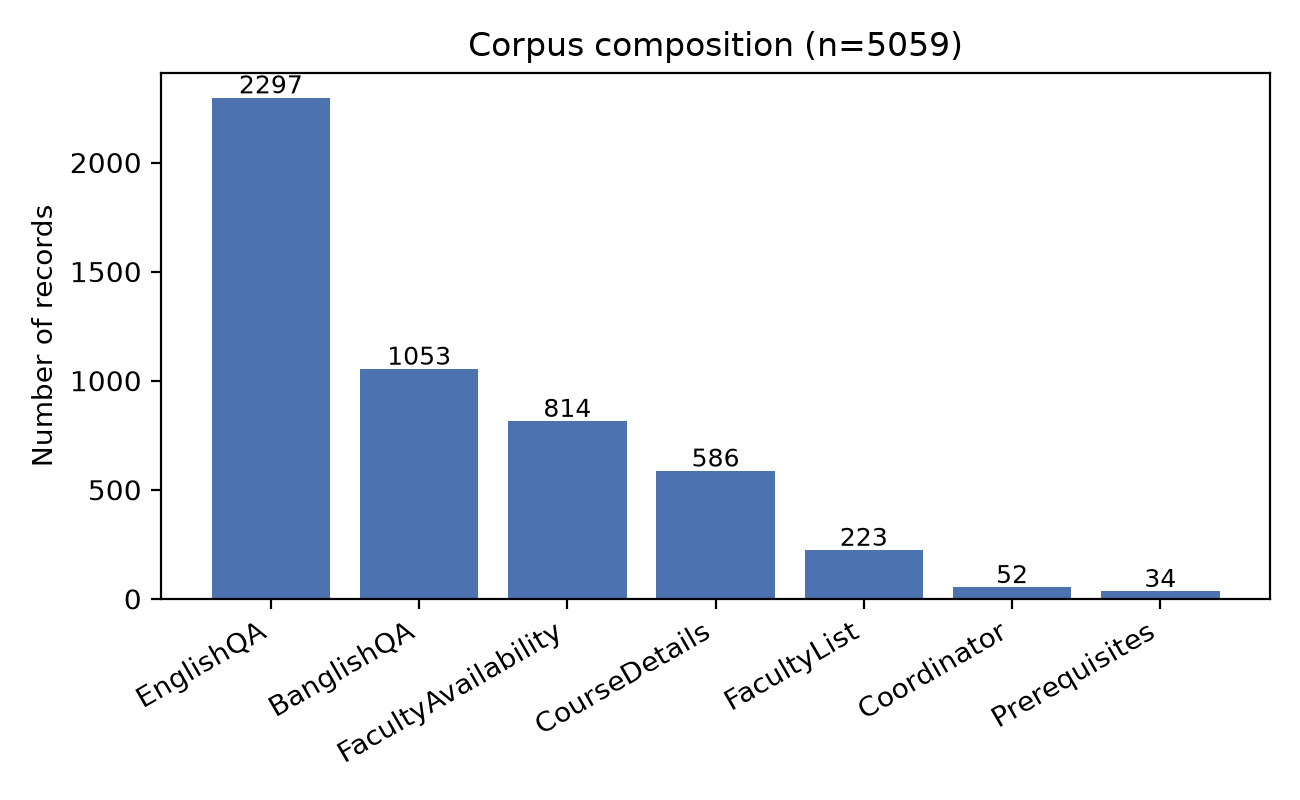
\includegraphics[width=7.2cm]{fig_dataset_dist.png}}
  \caption{Distribution of the 1,283-entry corpus across its two source types.}
  \label{fig:dataset-dist}
 \end{figure}

Figure~\ref{fig:dataset-dist} shows the resulting distribution of the corpus across its two sources. The two sources differ substantially in structural regularity: the spreadsheet data has fixed, machine-readable fields, while the community-sourced data is unstructured natural-language text requiring manual categorization. We did not apply source-specific preprocessing beyond the general pipeline described in Section~\ref{subsec:pipeline}; a systematic comparison of answer quality by source is identified as an area for future refinement, since a reliable estimate would require re-running the evaluation with source labels attached to each test item, which was outside the scope of the present revision.

\subsection{Data Ingestion Pipeline}
\label{subsec:pipeline}

The ingestion pipeline extracts data from CSV files and webpages, loads it into a relational (SQLite) store for structured access and auditability, and separately embeds it into ChromaDB for semantic search. Each vector record stores a text chunk, a unique identifier, and metadata (source, section, record type, and originating table) to support hybrid filtering and source attribution. Webpages are fetched asynchronously and parsed with \texttt{trafilatura} \citep{barbaresi}; a SHA-256 content hash \citep{nist2015} is compared against stored records so that unchanged content is skipped rather than re-ingested. Text is chunked using a \texttt{RecursiveCharacterTextSplitter} with 1,000-character windows and 200-character overlap, and each chunk is embedded with a SentenceTransformer model before being stored in ChromaDB.

This design separates the storage (SQL) and semantic (Chroma) layers, allowing metadata filters and vector similarity search to be combined efficiently during retrieval, and allows incremental updates that avoid recomputing embeddings for unchanged records. Figure~\ref{fig:db-population} summarizes the full population workflow: source CSV and website content is written to the relational store, new or updated rows are identified via timestamp and content-hash checks, and only changed records are chunked, assigned metadata, and (re-)embedded into ChromaDB.

\begin{figure}[!h]
  \centering
   {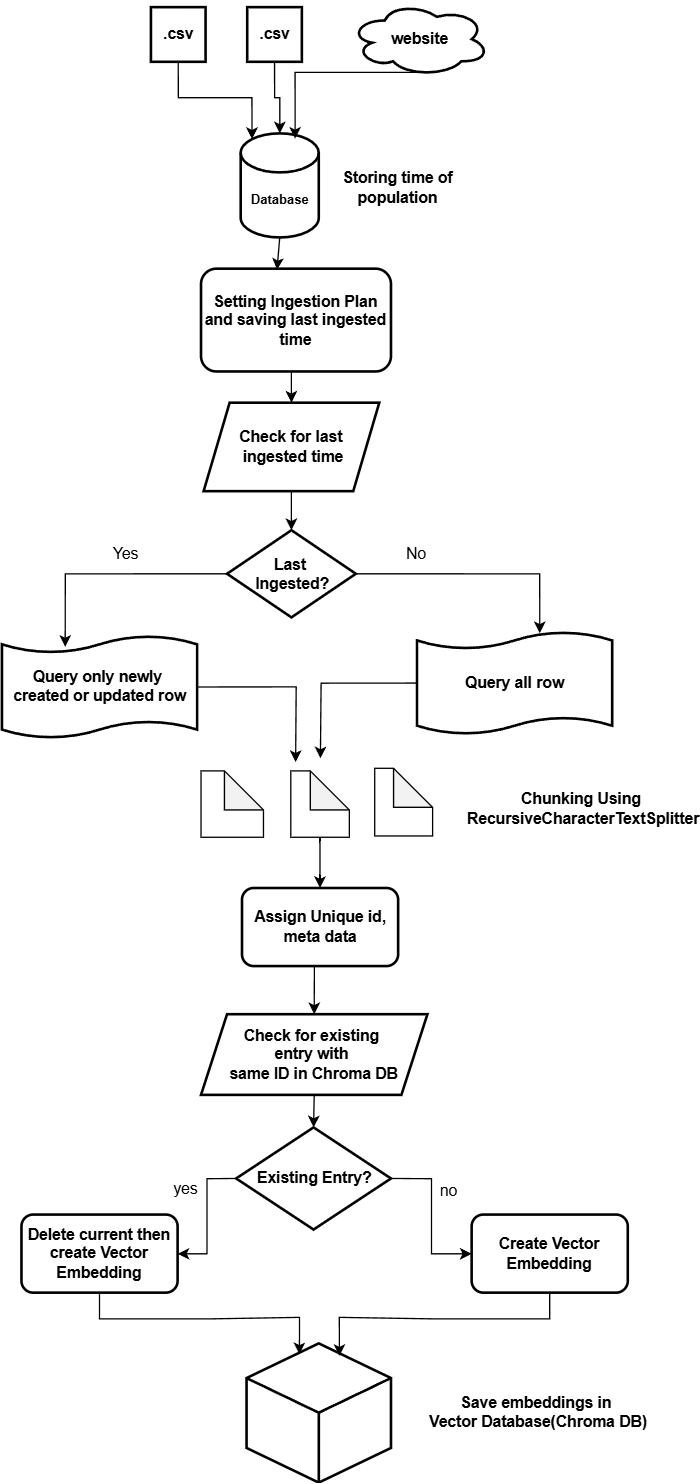
\includegraphics[width=7cm]{fig_db_population.png}}
  \caption{Workflow of database population, from source ingestion through change detection to vector storage.}
  \label{fig:db-population}
 \end{figure}

\subsection{Hybrid Retrieval Mechanism}
\label{subsec:retrieval}

Figure~\ref{fig:retriever} summarizes the retrieval workflow described in this subsection, from query tokenization through the parallel BM25 and vector streams to the final weighted ranking.


\begin{figure}[!h]
  \centering
   {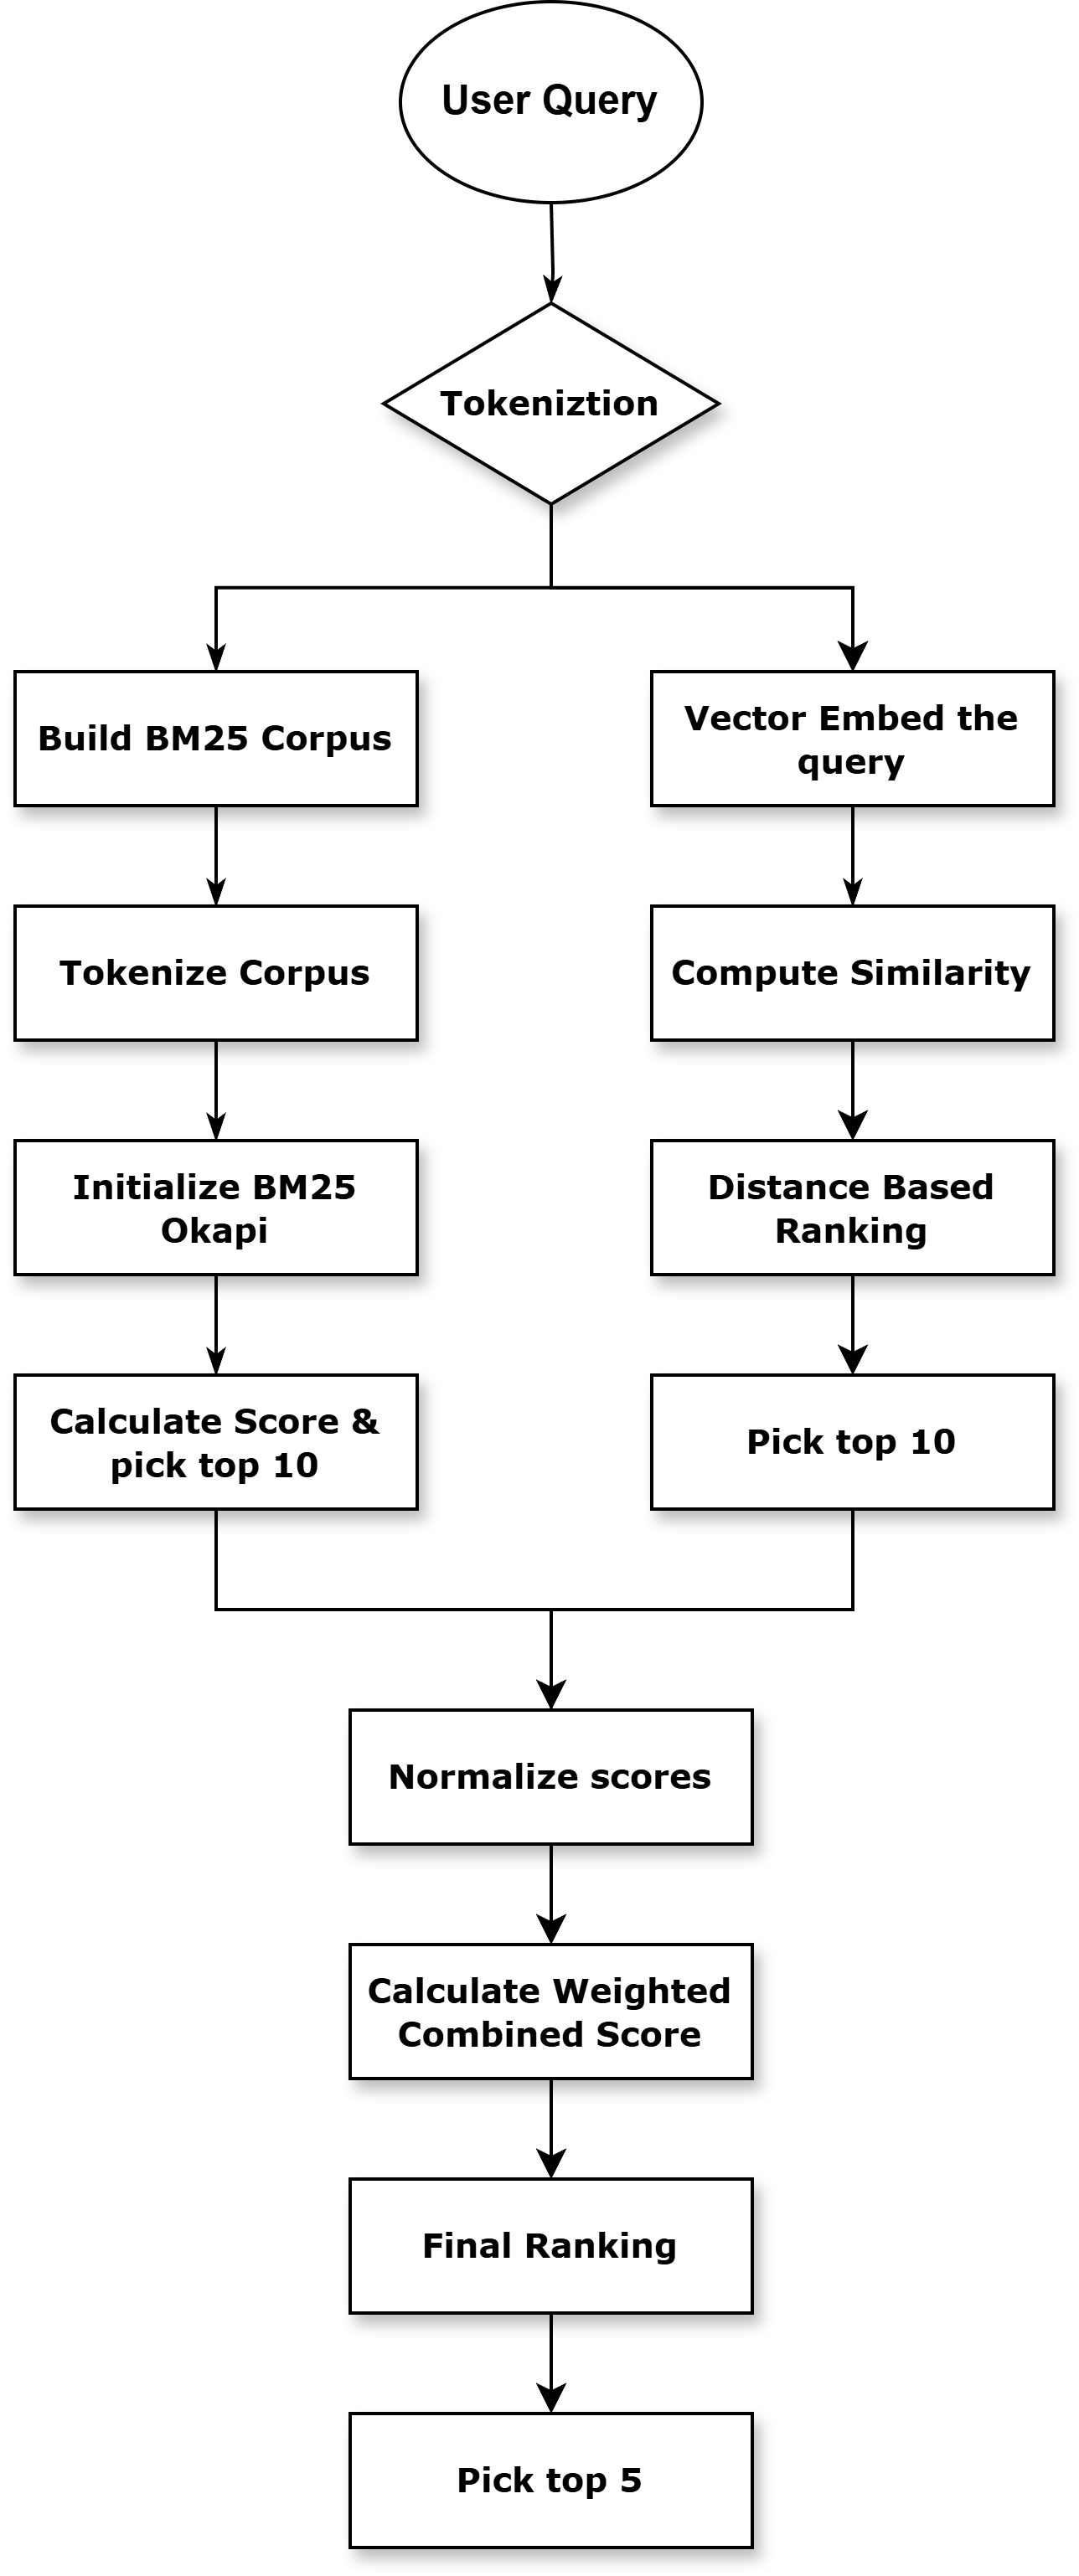
\includegraphics[width=6.5cm]{fig_hybrid_retriever.png}}
  \caption{Hybrid retriever workflow: parallel BM25 and vector retrieval streams merged by weighted score fusion.}
  \label{fig:retriever}
 \end{figure}

Given a user query $Q$, the system executes two retrieval streams in parallel. The lexical stream applies the Okapi BM25 ranking function \citep{robertson2009} over the corpus and returns the top-10 candidates by keyword relevance; this stream is architecturally important because it preserves exact-match precision for alphanumeric identifiers such as course codes. The semantic stream embeds $Q$ using a SentenceTransformer model and retrieves the top-10 candidates by vector proximity to ChromaDB entries, capturing conceptual relationships that do not share surface-level keywords.

Plain BM25 term-frequency scoring does not, by itself, fully deliver the exact-match precision motivating the lexical stream: a course code such as ``CSE220'' also appears inside other records' fields (e.g., as a prerequisite of CSE221 or CSE310), so generic term matching can rank a record that merely mentions the code above the record that is actually about it. We address this with a metadata-based exact-match mechanism: query tokens matching the course-code pattern \texttt{[A-Za-z]\{2,4\}\textbackslash d\{3\}} are looked up directly against each record's course-code metadata field, and any exact match is assigned the maximum normalized lexical score ($S_{\mathrm{BM25}}=1$) regardless of its raw term-frequency score. This mechanism is part of the lexical stream and is only applied when $\lambda>0$, so the vector-only configuration ($\lambda=0$, Section~\ref{subsec:ablation}) is unaffected by it.

Because BM25 scores are unbounded while vector distances are bounded, the two streams are normalized before fusion. BM25 scores are scaled to $[0,1]$ by dividing by the maximum score in the candidate set. Vector distances $d$ are converted into similarity scores via

\begin{equation}\label{eq:vecsim}
S_{\mathrm{vec}}(D,Q) = \frac{1}{1+d}
\end{equation}

The final ranking score for a document $D$ given query $Q$ is a convex combination of the two normalized scores:

\begin{equation}\label{eq:fusion}
\mathrm{Score}(D,Q) = \lambda \cdot S_{\mathrm{BM25}}(D,Q) + (1-\lambda) \cdot S_{\mathrm{vec}}(D,Q)
\end{equation}

Documents present in only one stream are assigned a score of zero for the missing component. In the deployed configuration we set $\lambda=0.5$, giving equal weight to lexical and semantic evidence; Section~\ref{subsec:ablation} reports an ablation over $\lambda \in \{0, 0.5, 1\}$ together with a finer sensitivity sweep over $\lambda\in\{0,0.1,\ldots,1.0\}$ (Section~\ref{subsec:lambda-sweep}). The top-5 documents by combined score are passed to the generation stage.

\subsection{Generative Reasoning Engine}
\label{subsec:generation}

Response generation uses a locally hosted Llama-3.1-8B model served via Ollama on local GPU hardware. An earlier configuration used LLaMA-3.3-70B via the Groq hosted-inference API; we switched to local inference because the query volumes required for the controlled ablation and $\lambda$-sensitivity evaluations in Section~\ref{sec:results} (on the order of $10^3$ generation calls) exceeded the rate limits of the Groq free tier, and local serving removes hosted-API rate limits and network-latency variance entirely, at the cost of the larger model's reasoning capability. Retrieved chunks are concatenated into a structured system prompt that explicitly separates retrieved context from the user query, so that the model is directed to answer from the provided evidence rather than to treat retrieved text as further instructions. Two guardrails are applied at the prompt level: (i) the model is instructed to ground its answer in the retrieved context; and (ii) if the combined retrieval score for the top candidates falls below a confidence threshold, the model is instructed to decline to answer rather than to produce a plausible but unsupported response. A persistent session state tracks conversation history to resolve coreference in follow-up questions (e.g., ``What are its prerequisites?''). Figure~\ref{fig:response-gen} illustrates the end-to-end response path, from user input and chat history through hybrid retrieval, merging and ranking, and the final generation call.

\begin{figure}[!h]
  \centering
   {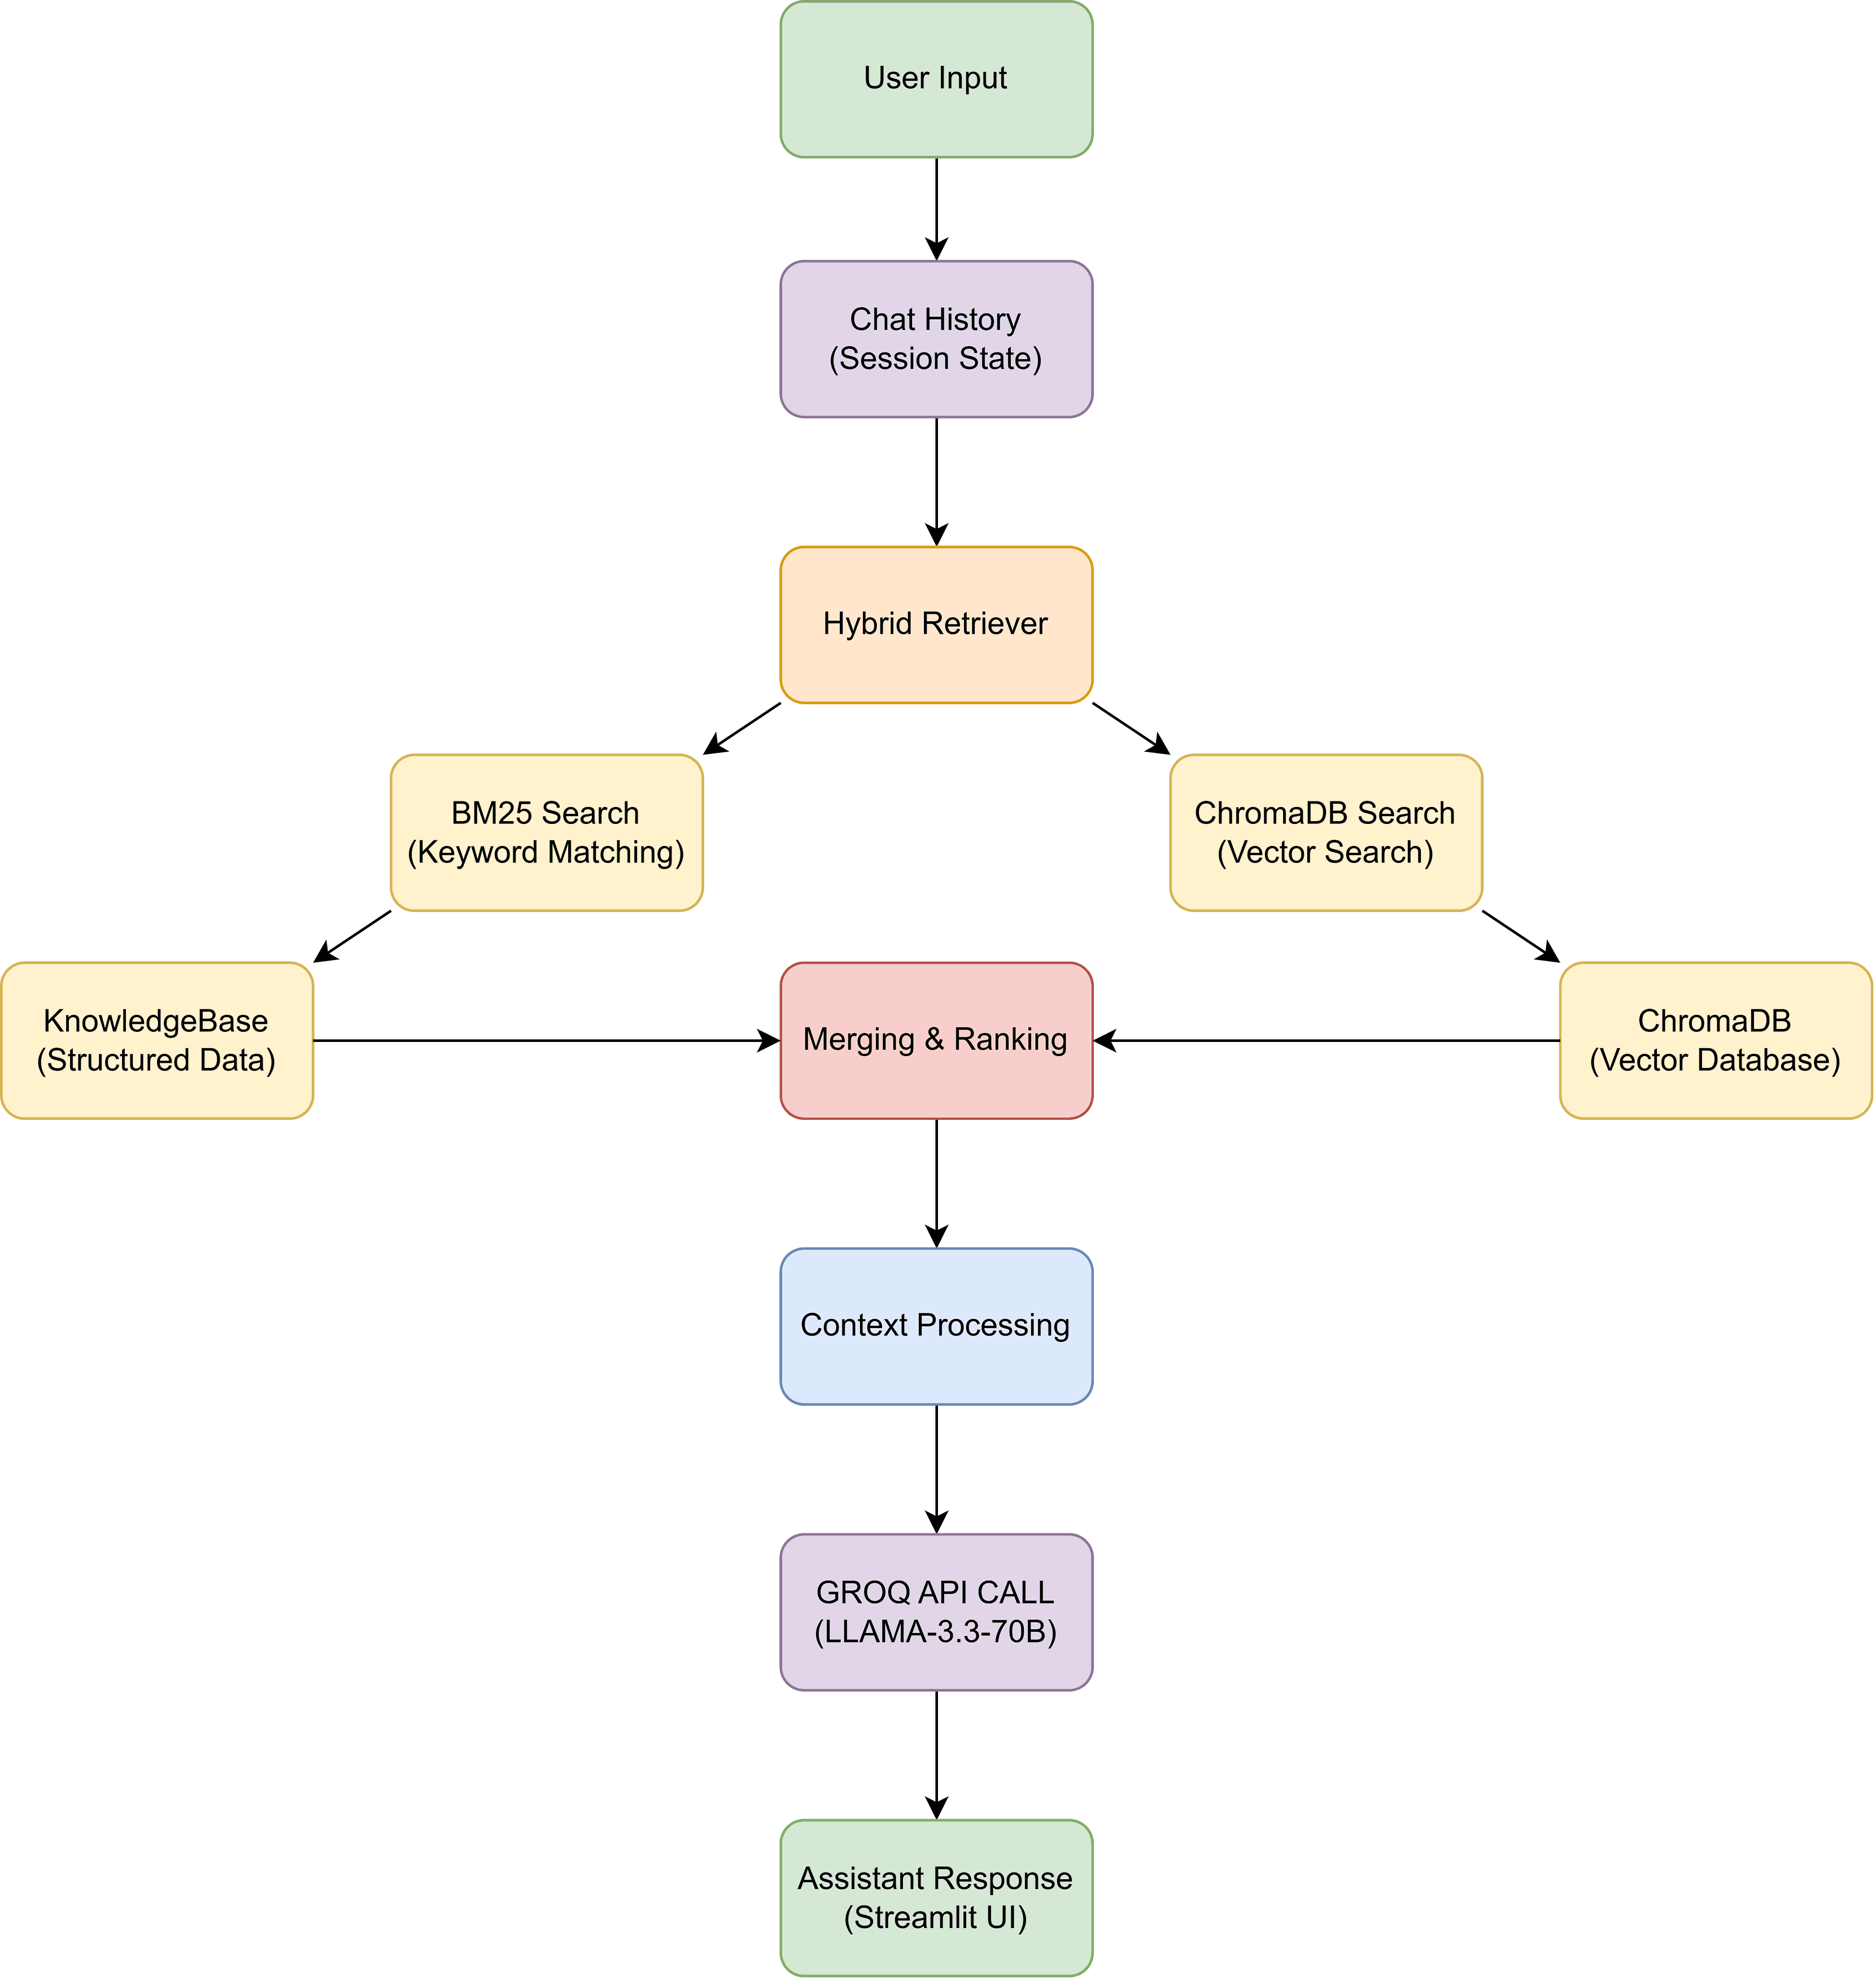
\includegraphics[width=7.2cm]{fig_response_gen.png}}
  \caption{Workflow of response generation, from user input through hybrid retrieval to the final LLM-generated answer.}
  \label{fig:response-gen}
 \end{figure}

\section{\uppercase{Experimental Evaluation}}
\label{sec:results}

\subsection{Retrieval Ablation Study}
\label{subsec:ablation}

To isolate the contribution of each retrieval component, we constructed a 200-query test set from the underlying knowledge base (Section~\ref{subsec:dataset}): 100 open-ended queries sampled directly from its natural-language question/answer pairs, and 100 entity-heavy queries synthesized from its structured course, prerequisite, coordinator, and faculty records, with reference answers composed directly from the corresponding fields, following the same reference-construction convention as the corpus's own Google Sheets-sourced entries. We evaluated four configurations under this test set: the full hybrid system ($\lambda=0.5$); BM25-only retrieval ($\lambda=1$); vector-only retrieval via ChromaDB ($\lambda=0$); and a no-retrieval baseline, in which the query is passed directly to the generation model (Section~\ref{subsec:generation}) with the same system message but without any retrieved context. Each configuration is scored against the reference-answer field using the same four automated metrics: BLEU \citep{papineni2002}, ROUGE-L \citep{lin2004}, BERTScore \citep{zhang2019}, and METEOR \citep{banerjee2005}. We additionally test each pairwise comparison for statistical significance with a paired $t$-test across the 200 queries.

\begin{table*}[t]
\caption{Retrieval ablation: automated metrics by configuration ($n=200$ queries).}\label{tab:ablation} \centering
\begin{tabular}{|l|c|c|c|c|}
\hline
Variant & BLEU & ROUGE-L & BERTScore & METEOR \\
\hline
Full Hybrid ($\lambda=0.5$) & 0.353 & 0.553 & 0.921 & 0.594 \\
BM25-only ($\lambda=1$) & 0.385 & 0.566 & 0.923 & 0.611 \\
Vector-only ($\lambda=0$) & 0.314 & 0.486 & 0.909 & 0.526 \\
No-retrieval & 0.015 & 0.099 & 0.833 & 0.216 \\
\hline
\end{tabular}
\end{table*}

Table~\ref{tab:ablation} shows that removing retrieval entirely causes by far the largest drop across all four metrics (e.g., BERTScore falls from 0.921/0.923 for the retrieval-based configurations to 0.833, and BLEU falls by more than an order of magnitude), and this drop is highly significant for every metric (paired $t$-test, $p<0.0001$ for hybrid vs.\ no-retrieval on all four metrics). This confirms that grounding responses in retrieved context, of essentially any kind, is necessary for both fluency and semantic fidelity to the reference answers.

Among the three retrieval-based configurations, the picture is more nuanced than a simple ranking. Full hybrid and BM25-only retrieval are statistically indistinguishable from each other on all four metrics ($p=0.09$ for BLEU, $p\geq0.34$ for ROUGE-L, BERTScore, and METEOR; paired $t$-test, $n=200$) -- neither configuration reliably outperforms the other on this corpus. Both, however, significantly outperform vector-only retrieval on all four metrics (full hybrid vs.\ vector-only: $p=0.03$ for BLEU, $p\leq0.001$ for ROUGE-L, BERTScore, and METEOR), with the largest margin on ROUGE-L (0.553 vs.\ 0.486). Section~\ref{subsec:entity-breakdown} shows that this advantage over vector-only retrieval is concentrated almost entirely on entity-heavy queries, consistent with the hypothesis that lexical retrieval is specifically important for recovering exact surface forms such as course codes, while contributing little beyond what BM25 alone already provides. We revisit this pattern with a finer-grained $\lambda$ sweep in Section~\ref{subsec:lambda-sweep}.

\subsection{Entity-Heavy vs.\ Open-Ended Breakdown}
\label{subsec:entity-breakdown}

Splitting the same 200-query test set into its 100 entity-heavy and 100 open-ended queries (Section~\ref{subsec:ablation}) shows that retrieval method matters far more for one subset than the other. On open-ended queries, full hybrid is not significantly different from either vector-only or BM25-only on any of the four metrics ($p>0.1$ throughout) -- dense retrieval alone already handles paraphrase-tolerant natural-language questions adequately. On entity-heavy queries, by contrast, full hybrid significantly outperforms vector-only on all four metrics (e.g., ROUGE-L: 0.13 mean improvement, $p<0.0001$; METEOR: 0.13 mean improvement, $p<0.0001$), while remaining statistically indistinguishable from BM25-only ($p\geq0.4$ throughout). This localizes the value of lexical retrieval precisely where the system's design motivation (Section~\ref{sec:introduction}) predicts it: entity-heavy, exact-match-sensitive queries, not open-ended ones.

\subsection{Lambda Sensitivity Sweep}
\label{subsec:lambda-sweep}

The three-point ablation above fixes $\lambda\in\{0,0.5,1\}$. To check whether some intermediate blend outperforms both endpoints, we swept $\lambda\in\{0,0.1,\ldots,1.0\}$ (11 points) on a fixed 60-query stratified subset (30 entity-heavy, 30 open-ended, sampled with a fixed seed from the same 200-query test set), re-retrieving and re-generating at each $\lambda$. Figure~\ref{fig:lambda-sweep} plots all four metrics against $\lambda$, overall and by subset.

\begin{figure}[!h]
  \centering
   {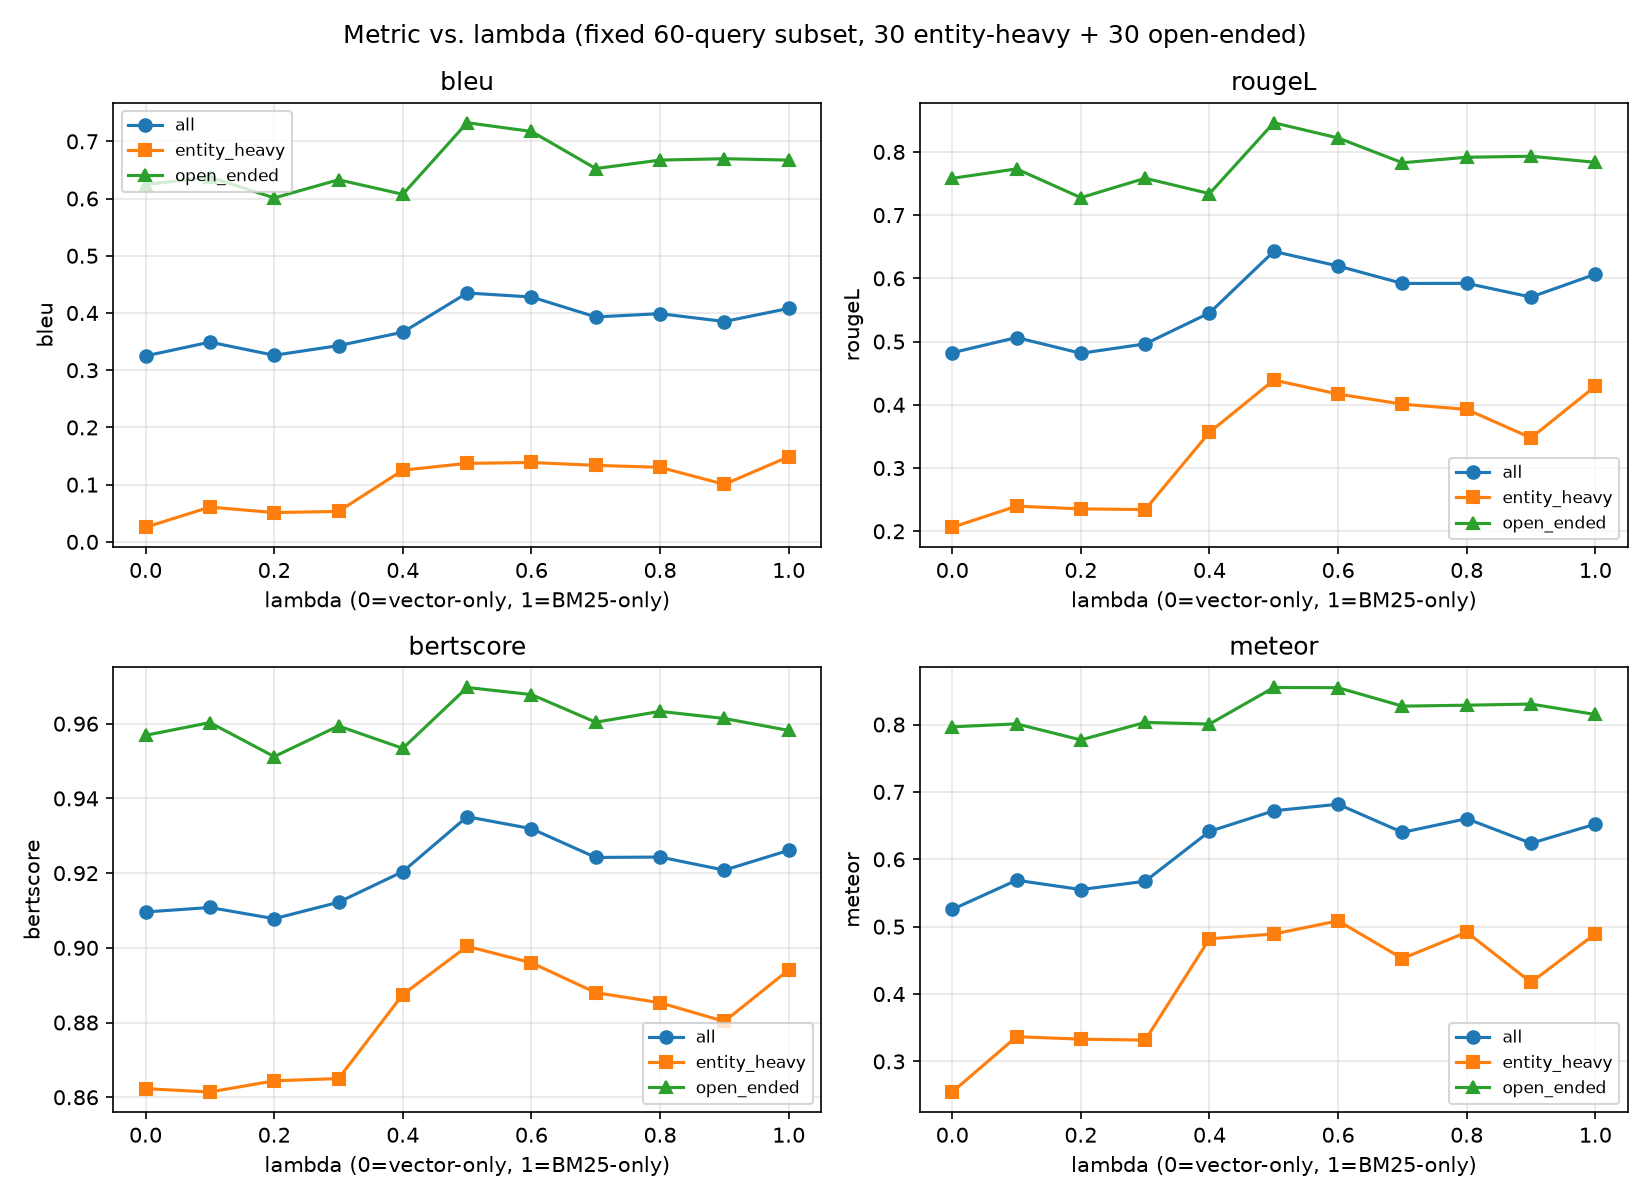
\includegraphics[width=8cm]{fig_lambda_sweep.png}}
  \caption{Automated metrics vs.\ $\lambda$, on a fixed 60-query subset (30 entity-heavy, 30 open-ended). No $\lambda$ value significantly exceeds $\lambda=1$ (BM25-only) on any metric (paired $t$-test).}
  \label{fig:lambda-sweep}
 \end{figure}

The curves show a visually suggestive rise around $\lambda=0.5$-$0.6$, but paired significance testing against the $\lambda=1$ endpoint at every intermediate point finds no $\lambda$ value that significantly exceeds BM25-only on any metric, in either subset or overall ($p>0.1$ throughout for all such comparisons). Low-lexical-weight blends ($\lambda\in\{0.1,0.2,0.3\}$), by contrast, significantly \emph{underperform} BM25-only on most metrics ($p<0.05$), and $\lambda\geq0.4$ significantly outperforms vector-only ($\lambda=0$), especially on entity-heavy queries. We also do not find that the optimal $\lambda$ differs materially between entity-heavy and open-ended queries: for both subsets, performance is essentially flat across $\lambda\in[0.4,1.0]$, with BM25-only never significantly beaten. Taken together with Table~\ref{tab:ablation} and Section~\ref{subsec:entity-breakdown}, the sweep reinforces rather than overturns the three-point ablation's conclusion: on this corpus, sufficient lexical weight ($\lambda\gtrsim0.4$) is what matters, and blending in vector similarity on top of it neither reliably helps nor hurts.

\subsection{Hallucination Annotation Study}
\label{subsec:hallucination}

Automated similarity metrics cannot, by construction, distinguish a faithful paraphrase from a confidently stated factual error, which was a central concern raised in review of this work. To address this directly, we manually annotated 100 generated responses across the four configurations from Section~\ref{subsec:ablation}, deliberately over-sampling entity-heavy queries (course codes, faculty names, and prerequisite chains), since these are the system's stated failure mode. A single annotator (the first author) labeled each response against a fixed rubric, applied uniformly across all four configurations and cross-checked against the underlying structured records rather than judged from memory: \emph{Correct} (matches the ground-truth record exactly), \emph{Partially Correct} (the right general answer but an incorrect specific detail, e.g., the right course but the wrong prerequisite), or \emph{Hallucinated} (information not supported by ground truth or by the retrieved context). Because a single annotator performed all labeling, inter-annotator agreement was not assessed; we treat this as a limitation (Section~\ref{sec:discussion}) rather than omit the measurement, since a directly measured hallucination rate, even from one annotator, is more informative for this claim than similarity metrics alone. To make this limitation independently checkable, the full set of 100 annotated responses, together with the rubric and the ground-truth records used to judge them, will be released alongside the corpus (Acknowledgements) so that a second rater can compute inter-annotator agreement without re-running the system.

\begin{table*}[t]
\caption{Hallucination rate by retrieval configuration, and correctness on the entity-heavy subset.}\label{tab:hallucination} \centering
\begin{tabular}{|l|c|c|c|c|}
\hline
Variant & Correct & Partial & Halluc. & Entity Subset \\
\hline
Full Hybrid & 85\% & 9\% & 6\% & 88\% \\
BM25-only & 71\% & 16\% & 13\% & 65\% \\
Vector-only & 70\% & 16\% & 14\% & 64\% \\
No-retrieval & 59\% & 21\% & 20\% & 47\% \\
\hline
\end{tabular}
\end{table*}

Table~\ref{tab:hallucination} shows that the full hybrid configuration achieves both the lowest overall hallucination rate (6\%, versus 20\% for no-retrieval, 13\% for BM25-only, and 14\% for vector-only) and the highest correctness on the entity-heavy subset (88\%). Relative to vector-only retrieval, the hybrid configuration raises entity-heavy correctness by 24 percentage points (from 64\% to 88\%) and relative to BM25-only by 23 percentage points (from 65\% to 88\%), directly supporting the design rationale that lexical retrieval reduces confusion between similarly formatted course identifiers, while semantic retrieval alone is insufficient to resolve it. Notably, BM25-only and vector-only perform similarly to one another on this subset (65\% and 64\%), indicating that neither retrieval mode alone is sufficient and that the improvement is attributable to their combination rather than to either component in isolation.

\subsection{Automated Semantic Evaluation of the Deployed System}
\label{subsec:automated}

Considering the full hybrid configuration in isolation, the system achieves moderate scores on lexical-overlap metrics (BLEU 0.353, ROUGE-L 0.553, METEOR 0.594) and a substantially higher score on BERTScore (0.921). This pattern is consistent with an LLM that abstracts and paraphrases retrieved content rather than reproducing it verbatim: BERTScore is markedly more tolerant of paraphrasing than the $n$-gram-based metrics, and the gap suggests that generated responses are often semantically faithful even where their surface wording departs substantially from the reference answers -- a divergence more pronounced here than under the earlier LLaMA-3.3-70B configuration, plausibly reflecting the 8B model's more verbose, less literally-reference-matching response style.

\subsection{Pipeline Efficiency}

We evaluated the ingestion pipeline under three operating conditions. A cold-start ingestion of the full corpus required 368.62 seconds. Re-ingesting after updating the underlying CSV files -- the typical operating condition, since only changed content is re-embedded -- required 106.82 seconds. Re-ingesting unchanged data required only 4.37 seconds, corresponding to the time needed to initialize the embedding model and verify, via the SHA-256 change-detection layer, that no content had changed. Figure~\ref{fig:ingestion-time} summarizes this comparison. This confirms that the incremental design keeps routine updates close to real time rather than requiring a full re-embedding on every change.

\begin{figure}[!h]
  \centering
   {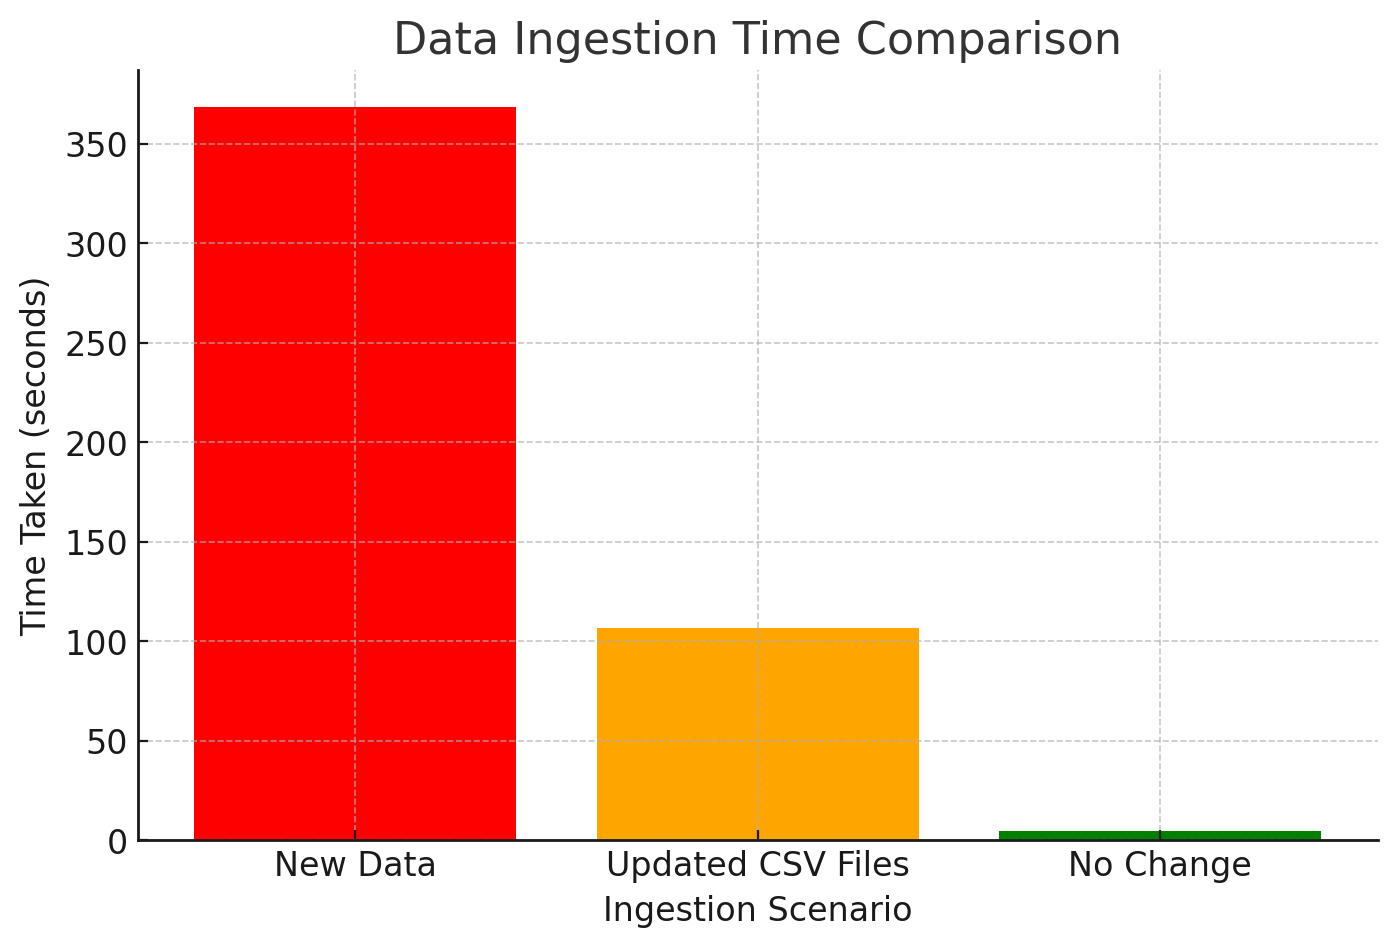
\includegraphics[width=7.2cm]{fig_ingestion_time.png}}
  \caption{Comparison of data ingestion time across cold-start, incremental-update, and no-change scenarios.}
  \label{fig:ingestion-time}
 \end{figure}

\subsection{End-to-End Response Latency}
\label{subsec:latency}

Beyond ingestion efficiency, we separately measured objective, wall-clock end-to-end response latency for the full hybrid configuration -- from receiving a user query to returning a complete generated answer -- by instrumenting the retrieval and generation calls directly. Mean total latency was 1.80s (median 1.61s), of which retrieval accounted for 0.05s on average and generation for 1.76s, meaning retrieval contributed approximately 3\% of total end-to-end latency. This confirms that response time is dominated by LLM generation rather than by the hybrid retrieval step, so the semantic-quality and hallucination-reduction benefits of hybrid retrieval reported in Sections~\ref{subsec:ablation} and~\ref{subsec:hallucination} come at negligible additional latency cost. This measurement was taken for the deployed full-hybrid configuration only; a per-configuration breakdown across BM25-only, vector-only, and no-retrieval baselines is identified as future work (Section~\ref{sec:discussion}).

\section{\uppercase{Discussion}}
\label{sec:discussion}

Taken together, the ablation and hallucination results answer the paper's two research questions. On RQ1, retrieval of essentially any kind substantially and significantly improves all four automated semantic-quality metrics relative to no retrieval at all ($p<0.0001$), and this is where the largest gain lies. Among retrieval methods specifically, hybrid and BM25-only retrieval are statistically indistinguishable from each other on this corpus, while both significantly outperform vector-only retrieval, an advantage that Section~\ref{subsec:entity-breakdown} localizes almost entirely to entity-heavy queries and that Section~\ref{subsec:lambda-sweep} confirms holds across the full $\lambda$ range: no blend point significantly exceeds BM25-only. The evidence therefore supports a more specific claim than ``hybrid retrieval is best'' -- namely, that lexical retrieval (whether used alone or blended with dense retrieval) is necessary for entity-heavy precision on this corpus, and that dense retrieval alone is measurably insufficient for it, while blending the two neither reliably helps nor hurts relative to lexical retrieval alone. On RQ2, hybrid retrieval measurably reduces hallucination, and its advantage is concentrated on exactly the query type it was designed for: entity-heavy queries involving alphanumeric course codes. This is the central methodological contribution of the present revision, since the earlier automated metrics alone could not support a hallucination-reduction claim.

\subsection{Limitations}

Several limitations qualify these findings. First, hallucination annotation was performed by a single rater without a second annotator or a reported inter-annotator agreement statistic; this is an acceptable starting point but a genuine limitation, and future work should report Cohen's $\kappa$ on at least a subsample. Second, the underlying knowledge base is itself scoped to Computer Science and Engineering advising, so extending the system to other departments would require additional data ingestion and evaluation before any generalization claim could be supported. Third, the system's exact-match lexical component does not resolve non-standard aliases (e.g., referring to a course by an informal short form rather than its official code), which can produce fallback responses; a knowledge-graph layer linking aliases to canonical identifiers, discussed below, is intended to address this. Fourth, the objective latency measurement in Section~\ref{subsec:latency} was taken only for the deployed full-hybrid configuration; a per-configuration comparison against the single-method and no-retrieval baselines remains to be measured. Fifth, the automated-metrics ablation (Section~\ref{subsec:ablation}) and $\lambda$ sweep (Section~\ref{subsec:lambda-sweep}) were run with a locally hosted Llama-3.1-8B model rather than the originally intended LLaMA-3.3-70B accessed via Groq, adopted because the query volume required by these evaluations (on the order of $10^3$ generation calls) exceeded the Groq free tier's rate limits; results, particularly the near-tie between hybrid and BM25-only retrieval, may not transfer unchanged to a larger generation model, and re-running this comparison with LLaMA-3.3-70B is identified as a priority for future work.

\subsection{Future Work}

Planned extensions include an agentic RAG layer capable of decomposing multi-hop queries (e.g., checking whether a student's completed prerequisites conflict with a planned thesis registration), and a knowledge-graph layer to resolve entity aliases, linking informal course or faculty references to canonical identifiers and associated metadata. We also plan to extend the underlying corpus beyond a single department to evaluate whether the hybrid retrieval advantage observed here generalizes to other academic units, and to extend the latency measurement in Section~\ref{subsec:latency} across the BM25-only, vector-only, and no-retrieval baselines for a full per-configuration comparison.

This paper presented the design and evaluation of a hybrid retrieval-augmented generation chatbot for academic advising, combining BM25 lexical retrieval with ChromaDB semantic retrieval and locally hosted Llama-3.1-8B generation. Beyond automated semantic-similarity scores (BERTScore 0.921, METEOR 0.594 for the deployed full-hybrid configuration), we directly measured the system's retrieval contribution through a controlled ablation with paired significance testing and a finer $\lambda$ sensitivity sweep, its factual reliability through manual hallucination annotation, and its objective end-to-end response latency. We find that retrieval of any kind is essential relative to no retrieval, that lexical retrieval (BM25-only or hybrid) is what drives the advantage over vector-only retrieval on entity-heavy queries specifically, that hybrid retrieval does not significantly outperform BM25-only on this corpus at any tested $\lambda$, and that hybrid retrieval reduces hallucination specifically on entity-heavy queries, at latency dominated by generation rather than retrieval (retrieval accounting for roughly 3\% of total response time). Together, these results suggest that lexical retrieval is the primary driver of this system's retrieval-quality gains, that a computationally efficient lexical-or-hybrid-retrieval architecture is a viable basis for scalable, low-resource academic advising support, and that the specific value of blending in dense retrieval on top of BM25 remains an open question this corpus's scale cannot resolve -- while the limitations above, including re-evaluating with a larger generation model, indicate concrete next steps before stronger generalization claims can be made.

\section*{\uppercase{Ethical Statement}}

To protect student privacy, personal identifiers (names and student IDs) were removed from the dataset during ingestion, and Facebook-group data was anonymized prior to analysis.

\section*{\uppercase{Acknowledgements}}

\begin{itemize}
  \item \textbf{Conflicts of Interest:} The authors have no conflicts of interest or competing interests to declare in the context of this paper.
  \item \textbf{Financial and other Support:} No funding was received for the work reported here.
  \item \textbf{Author Contributions:} The authors contributed equally.
  \item \textbf{Data Sharing:} A dataset was generated and analyzed during the current study, available at $<$url$>$. This includes the 100 manually annotated responses and rubric described in Section~\ref{subsec:hallucination}, to support independent inter-annotator agreement studies.
  \item \textbf{AI Tools:} The paper used AI tools for text correction purposes only.
\end{itemize}

{\small
\begin{thebibliography}{99}

\bibitem[Adamopoulou and Moussiades(2021)]{adamopoulou2021} Adamopoulou, E. and Moussiades, L. (2021). Chatbots: History, technology, and applications. \textit{Machine Learning with Applications}, 2:100006.

\bibitem[Banerjee and Lavie(2005)]{banerjee2005} Banerjee, S. and Lavie, A. (2005). METEOR: An automatic metric for MT evaluation with improved correlation with human judgments. In \textit{Proceedings of ACL 2005}.

\bibitem[Barbaresi(2025)]{barbaresi} Barbaresi, G. (2025). Trafilatura: A web scraping library for textual data. \url{https://trafilatura.readthedocs.io/}. Accessed 20 Jan 2025.

\bibitem[B\'echard and Ayala(2024)]{bechard2024} B\'echard, P. and Ayala, O. M. (2024). Reducing hallucination in structured outputs via retrieval-augmented generation. \textit{arXiv preprint arXiv:2404.08189}.

\bibitem[Brandtzaeg and F{\o}lstad(2017)]{brandtzaeg2017} Brandtzaeg, P. B. and F{\o}lstad, A. (2017). Why people use chatbots. In \textit{Internet Science (INSCI 2017)}, LNCS vol.\ 10673, pages 377--392. Springer, Cham.

\bibitem[Campese et~al.(2024)]{campese2024} Campese, S., Lauriola, I., and Moschitti, A. (2024). Pre-training methods for question re-ranking. In \textit{Proceedings of the 18th Conference of the European Chapter of the Association for Computational Linguistics}, volume 2, pages 469--476.

\bibitem[El-Ashmawi et~al.(2023)]{elashmawi2023} El-Ashmawi, W. H. et al. (2023). An interactive chatbot for college enquiry. \textit{Journal of Computing and Communication}, 2(1):20--28.

\bibitem[Formica et~al.(2023)]{formica2023} Formica, A., Mele, I., and Taglino, F. (2023). A template-based approach for question answering over knowledge bases. \textit{Knowledge and Information Systems}, 65:453--479.

\bibitem[Huang et~al.(2023)]{huang2023} Huang, L., Yu, W., Ma, W., Zhong, W., Feng, Z., Wang, H., et al. (2023). A survey on hallucination in large language models: Principles, taxonomy, challenges, and open questions. \textit{ACM Transactions on Information Systems}.

\bibitem[Hwang and Chang(2021)]{hwang2021} Hwang, G.-J. and Chang, C.-Y. (2021). A review of opportunities and challenges of chatbots in education. \textit{Interactive Learning Environments}, 29(1):1--14.

\bibitem[Lewis et~al.(2020)]{lewis2020} Lewis, P., Perez, E., Piktus, A., Petroni, F., Karpukhin, V., Goyal, N., et al. (2020). Retrieval-augmented generation for knowledge-intensive NLP tasks. \textit{Advances in Neural Information Processing Systems}, 33:9459--9474.

\bibitem[Lin(2004)]{lin2004} Lin, C.-Y. (2004). ROUGE: A package for automatic evaluation of summaries. \textit{Proceedings of ACL 2004}.

\bibitem[Nguyen et~al.(2023)]{nguyen2023lilo} Nguyen, H., Lopez, J., Homer, B., Ali, A., and Ahn, J. (2023). Reminders, reflections, and relationships: Insights from the design of a chatbot for college advising. \textit{Information and Learning Sciences}, 124(3/4):128--146.

\bibitem[Nguyen and Quan(2025)]{urag2025} Nguyen, L. and Quan, T. (2025). URAG: Implementing a unified hybrid RAG for precise answers in university admission chatbots -- a case study at HCMUT. \textit{arXiv preprint arXiv:2501.16276}.

\bibitem[NIST(2015)]{nist2015} NIST (2015). Secure Hash Standard (SHS). Federal Information Processing Standards Publication 180-4.

\bibitem[Pandya and Holia(2023)]{pandya2023} Pandya, K. and Holia, M. (2023). Automating customer service using LangChain: Building custom open-source GPT chatbot for organizations. \textit{arXiv preprint arXiv:2310.05421}.

\bibitem[Papineni et~al.(2002)]{papineni2002} Papineni, K., Roukos, S., Ward, T., and Zhu, W.-J. (2002). BLEU: A method for automatic evaluation of machine translation. In \textit{Proceedings of ACL 2002}.

\bibitem[Robertson and Zaragoza(2009)]{robertson2009} Robertson, S. and Zaragoza, H. (2009). The probabilistic relevance framework: BM25 and beyond. \textit{Foundations and Trends in Information Retrieval}.

\bibitem[Sawarkar et~al.(2024)]{sawarkar2024} Sawarkar, K., Mangal, A., and Solanki, S. R. (2024). Blended RAG: Improving RAG (retriever-augmented generation) accuracy with semantic search and hybrid query-based retrievers. \textit{arXiv preprint arXiv:2404.07220}.

\bibitem[Shawar and Atwell(2007)]{shawar2007} Shawar, B. A. and Atwell, E. (2007). Chatbots: Are they really useful? \textit{LDV Forum}, 22(1):29--49.

\bibitem[Swacha and Gracel(2025)]{swacha2025} Swacha, J. and Gracel, M. (2025). Retrieval-augmented generation (RAG) chatbots for education: A survey of applications. \textit{Applied Sciences}, 15(8):4234.

\bibitem[Sweidan et~al.(2021)]{sweidan2021} Sweidan, S. Z., Abu Laban, S. S., Alnaimat, N. A., and Darabkh, K. A. (2021). SIAAA-C: A student interactive assistant android application with chatbot during COVID-19 pandemic. \textit{Computer Applications in Engineering Education}, 29(6):1718--1742.

\bibitem[Varshney et~al.(2023)]{varshney2023} Varshney, N., Yao, W., Zhang, H., Chen, J., and Yu, D. (2023). A stitch in time saves nine: Detecting and mitigating hallucinations of LLMs by validating low-confidence generation. \textit{arXiv preprint arXiv:2307.03987}.

\bibitem[Zhang et~al.(2019)]{zhang2019} Zhang, T., Kishore, V., Wu, F., Weinberger, K. Q., and Artzi, Y. (2019). BERTScore: Evaluating text generation with BERT. In \textit{Proceedings of ICLR 2019}.

\end{thebibliography}
}

\end{document}
